\chapter{Value Function Approximation in Reinforcement Learning}
In this chapter, we will focus on the study of function approximation for estimating state-value functions from on-policy data. That is, approximating $v_\pi$ from experience generated using a known policy $\pi$. The novelty in this chapter is that the approximate value function is not represented as a table, but as a parametrized functional form with a weight vector $\boldsymbol{w} \in \mathbb{R}^d$.

We will write $\hat{v}(s,\boldsymbol{w}) \approx v_\pi (s)$ for the approximate value of state $s$ given a weight vector $\boldsymbol{w}$, with $\hat{v}$ being either a linear function of the weights or, more generally, a (nonlinear) function computed by a multi-layer artificial neural network. Typically, the number of weights is much less than the number of states ($d \ll \left|\mathcal{S}\right|$) and changing one weight changes the estimated value of many states. Consequently, when a single state is updated, the change \textbf{generalizes} from that state to affect the values of many other states. Such generalization makes the learning potentially more powerful, but also potentially more difficult to manage and understand.

In addition to that, if the parametrized function form for $\hat{v}$  does not allow the estimated value to depend on certain aspects of the state, it will behave as if those aspects are unobservable to the agent, making it \textbf{possible to apply these techniques to partially observable problems} as well.

\section{Value function approximation}
Until now, we have seen methods that performed updates to an estimated value function by shifting its value at particular states towards an ``update target'' for that state. Let us refer to an individual update by the notation $s \mapsto u$, where $s$ is the state updated and $u$ is the update target that $s$’s estimated value is shifted towards. For example, the Monte Carlo update for value prediction is $S_t \mapsto G_t$; the TD(0) update is instead $S_t \mapsto R_{t+1} \gamma \hat{v} \left( S_{t+1},\boldsymbol{w}_t \right)$.

It is natural to interpret each update as specifying an example of the desired input-output behavior of the value function. In a sense, the update $s \mapsto u$ means that the estimated value for state $s$ should be more like the update target $u$. If we were to perform this update in tabular methods, we would shift $s$’s estimated value a fraction of the way towards $u$, while leaving the values of the other states unchanged. Now we permit arbitrarily complex and sophisticated methods to implement the update, and updating at $s$ generalizes so that the estimated values of many other states are changed as well. Machine learning methods that learn to mimic input-output examples in this way are called \textbf{supervised learning methods}, and when the outputs are numbers, like $u$, the process is called \textbf{function approximation}.

Artificial neural networks (ANN) are widely used for approximating nonlinear functions, especially because of the guarantees that the \textbf{universal approximation theorem} (initially proven by George Cybenko in 1989) provides. Cybenko, in fact, showed that an ANN with a single hidden layer containing a large enough finite number of sigmoid units can approximate, on a compact region of the network’s input space, any continuous function to any degree of accuracy \cite{Cybenko1989ApproximationBS}.

\section{Stochastic Gradient Descent for function approximation}
We now develop in detail stochastic gradient descent (SGD) methods for function approximation. SGD methods are among the most widely used function approximation methods and are particularly well suited for online reinforcement learning.

To limit the complexity of the matter at hand, we will consider only the case in which we update our network using \textit{only one example at a time}. Let us recall the formula we introduced in the previous chapter for updating the weights using SGD (for batches of examples we can use the mini-batch SGD):

\begin{equation}
    w_j \leftarrow w_j + \Delta w_j = w_j - \eta \frac{\partial J}{\partial w_j}
    \label{eq:ch7-singlesgdupdate}
\end{equation}

Since we will be updating $\boldsymbol{w}$ at each of a series of discrete time steps, $t = 0, 1, 2, ...$, we modify our notation to include the time information as such:

\begin{equation}
    w_{j,t+1} \leftarrow w_{j,t} + \Delta w_{j,t} = w_{j,t} - \eta \frac{\partial J}{\partial w_{j,t}}
    \label{eq:ch7-singlesgdfunctionapproxupdate}
\end{equation}

Assuming that our loss function is represented by the \textbf{mean square error} shown here:

\begin{equation}
    J(\boldsymbol{w}) = \sum_{s \in \mathcal{S}} \big(U_t - \hat{v}(S_t, \boldsymbol{w}_t) \big)^2
    \label{eq:ch7-meansquareerrorfunction}
\end{equation}

--where $U_t$ is our \textbf{target} and $\hat{v}(S_t, \boldsymbol{w}_t)$ is our current estimate-- we will then obtain the following weight update formula:

\begin{equation}
    \begin{split}
        \boldsymbol{w}_{t+1} &\doteq \boldsymbol{w}_t - \frac{1}{2} \eta \nabla \big[ U_t - \hat{v}(S_t, \boldsymbol{w}_t) \big]^2 \\
        &= \boldsymbol{w}_t + \eta \big[ U_t - \hat{v}(S_t, \boldsymbol{w}) \big] \nabla \hat{v} (S_t, \boldsymbol{w}_t)
    \end{split}
    \label{eq:ch7-genericstatefunctionapproxssdweightupdate}
\end{equation}

Since the step-size parameter $\eta$ is chosen arbitrarily, we multiplied it by $\frac{1}{2}$ to cancel out the 2 that comes from the derivative.

\subsection{Semi-gradient one-step SARSA prediction}
The weight update rule we just introduced can be used to extend to state-action value functions the mathematical framework we discussed for state value functions . In this case, the update target $U_t$ will be an approximation of $q_\pi (S_t,A_t )$, making the gradient-descent update as such:

\begin{equation}
    \boldsymbol{w}_{t+1} = \boldsymbol{w}_t + \eta \big[ U_t - \hat{q}(S_t,A_t,\boldsymbol{w}_t) \big] \nabla \hat{q}(S_t,A_t,\boldsymbol{w}_t)
    \label{eq:ch7-genericqvaluefunctionapproxssdweightupdate}
\end{equation}

If we combine this formula with the one we introduced in equation \ref{eq:ch5-sarsaupdaterule}, we obtain the \textbf{episodic semi-gradient one-step SARSA} update rule:

\begin{equation}
    \boldsymbol{w}_{t+1} = \boldsymbol{w}_t + \eta \big[ R_{t+1} + \gamma \hat{q}(S_{t+1},A_{t+1},\boldsymbol{w}_t) - \hat{q}(S_t,A_t,\boldsymbol{w}_t) \big] \nabla \hat{q}(S_t,A_t,\boldsymbol{w}_t)
    \label{eq:ch7-sarsaqvaluefunctionapproxssdweightupdate}
\end{equation}

It is called semi-gradient because we are not really taking the ``real'' gradient, as it would require us to calculate the gradient of $U_t$ as well (simply speaking, we assume the output is not function of $\boldsymbol{w}_t$ even though it is). This is essential to avoid introducing too much complexity and, if the policy is constant, we still have guarantees of convergence.

\subsection{Semi-gradient one-step SARSA control}
As usual, however, we are more interested in the problem of \textit{control}, rather than the one of \textit{prediction}. To tackle it in the case of function approximation, we employ methods that are essentially the same as the ones we used in the tabular case: for each possible action $a$ available in the current state $S_t$, we can compute $\hat{q}(S_t,a,\boldsymbol{w}_t)$ and then find the greedy action using:

\begin{equation*}
    A_{t}^{*} = \argmax_a \hat{q}(S_t,a,\boldsymbol{w}_t)
\end{equation*}

Policy improvement is then done by changing the estimation policy to a soft approximation of the greedy policy (e.g., $\varepsilon$-greedy policy). Since we are in the \textit{on-policy} case, actions are selected according to this same policy. We introduce the pseudo-code for the \textbf{episodic semi-gradient on-policy SARSA algorithm} in the box below:

\begin{algorithm}[H]
\DontPrintSemicolon
\SetAlgoVlined
\KwIn{a differentiable action-value function parametrization $\hat{q}: \mathcal{S} \times \mathcal{A} \times \mathbb{R}^d \rightarrow \mathbb{R}$}
\Parameters{step size $\eta > 0$, small $\varepsilon > 0$}
\Initialize{value-function weights $\boldsymbol{w} \in \mathbb{R}^d$ arbitrarily (e.g., $\boldsymbol{w = 0}$)}

 \Loop{for each episode}{
    $S, A \leftarrow$ initial state and action of episode (e.g., $\varepsilon$-greedy)\;
    \Loop{for each step of the episode}{
        Take action $A$, observe $R, S'$\;
        \If{$S'$ is terminal}{
            $\boldsymbol{w} \leftarrow \boldsymbol{w} + \eta \big[ R - \hat{q}(S,A,\boldsymbol{w})\big] \nabla \hat{q}(S,A,\boldsymbol{w})$\;
            Go to next episode\;
        }
        Choose $A'$ as a function of $\hat{q}(S',\cdot,\boldsymbol{w})$ (e.g., $\varepsilon$-greedy)\;
        $\boldsymbol{w} \leftarrow \boldsymbol{w} + \eta \big[ R + \gamma\hat{q}(S',A',\boldsymbol{w}) - \hat{q}(S,A,\boldsymbol{w})\big] \nabla \hat{q}(S,A,\boldsymbol{w})$\;
        $S \leftarrow S'$\;
        $A \leftarrow A'$\;
    }
 }
\caption{Episodic Semi-gradient SARSA for estimating $\hat{q} \approx q_*$}
\end{algorithm}

\subsection{Semi-gradient off-policy Q-learning}
The same thought process can be applied to obtain \textbf{semi-gradient Q-learning}, in which the update rule will be:

\begin{equation}
    \boldsymbol{w}_{t+1} = \boldsymbol{w}_t + \eta \big[ R_{t+1} + \gamma \argmax_a  \hat{q}(S_{t+1},a,\boldsymbol{w}_t) - \hat{q}(S_t,A_t,\boldsymbol{w}_t) \big] \nabla \hat{q}(S_t,A_t,\boldsymbol{w}_t)
    \label{eq:ch7-qlearningqvaluefunctionapproxssdweightupdate}
\end{equation}

Where $\boldsymbol{w}_t$ is the vector of the network’s weights, $A_t$ is the action selected at time $t$, and $S_t$ and $S_{t+1}$ are the inputs to the network at their respective time steps.

\section{Deep Q-Network}
Semi-gradient Q-learning (or, interchangeably, \textbf{Deep Q-Network}, \textbf{DQN}) has been used to solve Atari games. It combines Q-Learning with a deep (convolutional) neural network, allowing, in this case, the conversion of the original frames from the 60Hz video feed ($210 \times 160$ pixels, 128 colors) in an $84 \times 84$ matrix of luminance values. Since movement is very important in videogames (e.g., what is the direction of the ball in a tennis match, what is its speed, etc.) and it cannot be necessarily inferred from a single frame, researchers decided to feed the network a stack of four frames at a time (making the input $84 \times 84 \times 4$). In addition to that, the rewards of the DQN have been restricted to be one of $\left\{-1,0,+1\right\}$. This has proven to yield better results (possibly) due to a reduction of instability (we learn more quickly if actions that are similar give us the same reward). More information on this can be found in \cite{mnih2013atari} and \cite{mnih2015humanlevel}. Let us now look at some key features of DQN.

We are in the \textbf{control problem}: we want to learn the optimal way to play a game. This, of course, means that the more we learn, the greedier will our policy have to be: once we are confident in our policy, we will have to start playing at the best of our abilities. The value of both $\varepsilon$ and the decay will be part of our \textbf{hyperparameters} and we will have to find their best value experimentally. In the examples cited before, $\varepsilon$ was set to decrease linearly over the first million frames and the network was trained using a mini-batch stochastic gradient with batches of 32 images (each made up of 4 frames), with changes proportional to the running average of the squares of gradients (RMSprop).

Another important thing that may be somewhat counterintuitive, is that the network is made to play all Atari games, and not necessarily any specific one: the output layer (as shown in figure \ref{fig:ch7-dqnschema}) will then always be made up of 18 nodes, even though only a subset may ever have values that are not 0.

\begin{figure}
    \centering
    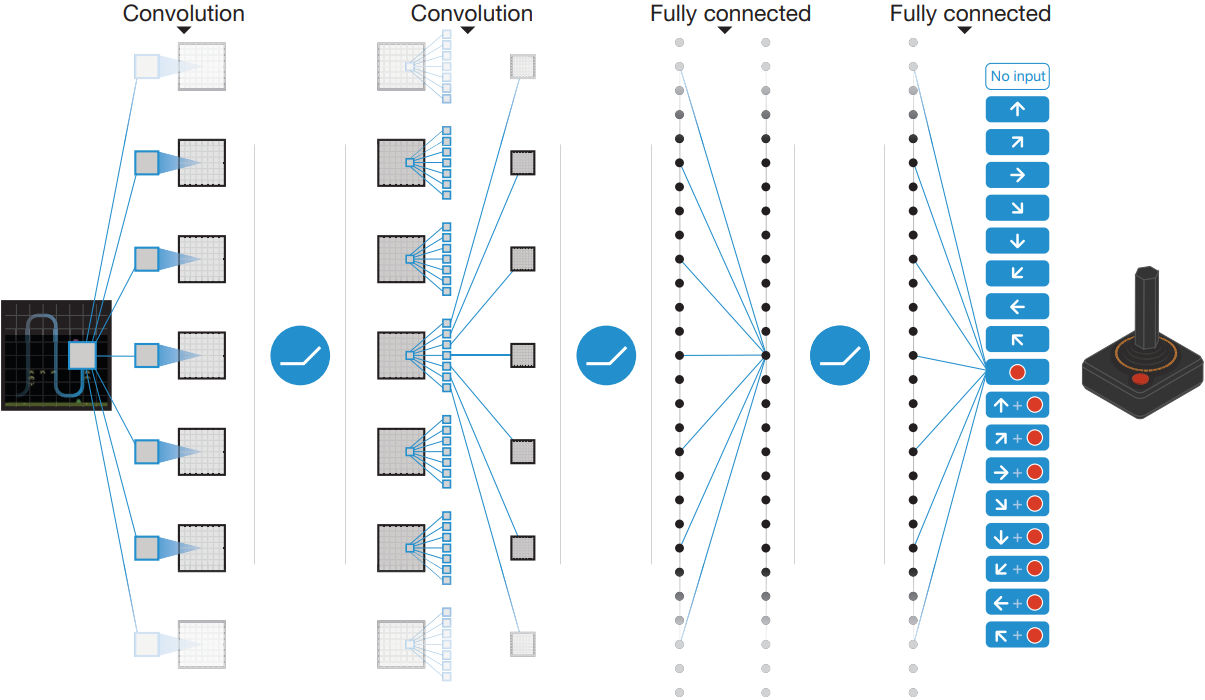
\includegraphics[scale=0.4]{Images/Chapter 7/ataridqn.png}
    \caption{DQN Schema}
    \source{Mnih et al. 2013}
    \label{fig:ch7-dqnschema}
\end{figure}

The authors of DQN made a series of changes to the ``standard'' Q-learning, the most important of which has probably been the introduction of \textbf{experience replay} to deal with the convergence problem of Q-learning. Picking actions that are highly correlated, in fact, has the effect of limiting our exploration of the space, thus leading to a much slower process of convergence (e.g., we may learn to run well on tarmac, but as soon as we go on sand, it will take us quite a while to adapt, causing updates with \textbf{high variance} to compensate).

The key idea is then to perform training through an \textbf{emulator} and storing the agent’s experience in a \textbf{replay memory} that is accessed to perform the weight updates. In practice, after the emulator executes action $A_t$ in a state represented by the image stack $S_t$, receiving reward $R_{t+1}$, we add to the replay memory (or \textbf{replay buffer}) a tuple made up of these values and the image stack $S_{t+1}$: $\big(S_t,A_t,R_{t+1},S_{t+1}\big)$. Each Q-learning update will then be performed by randomly sampling from the experience replay buffer. Instead of $S_{t+1}$ becoming the new $S_t$ for the next update, as it happens in normal Q-learning, a new, unconnected experience is drawn from the replay memory, helping us avoid getting stuck with actions that do not generalize. It is important to note that this is possible because Q-learning is an \textit{off-policy} algorithm, and so it does not need to learn from ``connected'' trajectories. More information can be found in \cite{10.1007/BF00992699}.